\documentclass{article}[12pt]
\usepackage[utf8]{inputenc}
\usepackage{graphicx}
%\graphicspath{{./figures/}}
\usepackage[utf8]{inputenc}
\usepackage[english]{babel}
\usepackage{amsmath}
\usepackage{natbib}

\newcommand{\possessivecite}[1]{\citeauthor{#1}'s \citeyear{#1}}
\author{}\title{Deep learning architectures in speech processing: Modeling dynamic speech gestures}

\begin{document}
\maketitle
\section{Introduction}
Deep learning as a broad framework of methods has taken speech and natural language processing system-building by a storm. The deluge of work that has happened in the last 25 or so years has shown remarkable promise, and growth. Therefore we don't need to underscore the need to present here the progress that has been made since the late 80's. One of the primary goals of our paper, therefore, is to highlight some of the most significant approaches and the findings therein. While our approach mostly will be chronological, we will also focus on how deep neural networks (DNN) have fundamentally revolutionized our approach to speech processing systems in general, and Automatic Speech Recognition (ASR) and Text-to-Speech Synthesis (TTS) in particular. More particularly, we will focus on a specific sub-task within broad speech processing and that is the articulatory-acoustic domain mapping. In that sense, the objective of this paper is to cover the most significant advances made in speech processing though deep learning models and architectures, but also focus on how deep learning architectures have helped unearth crucial generalizations between speech articulatory gestures and their acoustic manifestations. In addition, we want to focus on a very specific aspect within the use of DNNs in speech processing, namely the integration of linguistic knowledge in achieving some of the remarkable successes in the core tasks of speech processing. At the outset, we would like to outline that the goals of this paper are not to introduce the concepts of machine learning, but to specifically treat a class of learning algorithms that variously appear in the literature under the cover term deep learning. Essentially, all deep learning systems and architectures are a specific form of artificial neural networks which have been in existence for a significant amount of time, but regained currency in the mid-80s with publications emerging from the parallel distributed processing group at San Diego. The paper is organized as follows: In the following section, we motivate the need to look closely into the various deep learning initiatives and outline the importance of the major impacts of these learning mechanisms. In Section 3, we briefly, and very generally, discuss the various architectures that help build deep learning models. In section 4, we concentrate on a specific use-case and outline the successes in this use-case, namely, the articulatory-acoustic mapping problem. In section 5, we offer some perspective and perhaps, hazard some speculation as to the future of these learning models.

\section{Why Deep Learning?}
We will begin this section with \cite{manning2015} who in his paper points to a few crucial changes that have come as a consequence of the expansion of deep learning systems in natural language processing. One of his primary concerns and engagement in this paper has been to point out how natural language processing takes center stage as far as being one of the most important challenges for machine learning scientists and deep learning enthusiasts, alike. \possessivecite{manning2015} entreatment is a clarion call for linguists, NLP engineers and data scientists to shift focus away from beating benchmark dataset tasks and challenges, and to concentrate on ``problems, approaches, and architectures". The import of \possessivecite{manning2015} appeal to re-engage with the cognitive and design goals of the study of human languages has been felt and responded to by work that has sought to understand deep learning architectures in the context of language cognition, and essentially has managed to re-center focus on NLP tasks as not just an engineering challenge, but also to re-imagine the goals of NLP research broadly within the cognitive and language sciences. In this paper, and especially \ref{section 4}, we discuss in detail how these goals have been achieved, and in which direction NLP research is moving armed with deep learning tools. We will treat the use of deep learning methods on solving acoustic variation problems that come about of an essentially non-linear problem that of articulatory-acoustic mapping and articulatory-acoustic inversion. The non-linearities that arise in the articulatory-acoustic mapping are a direct consequence of the way speech articulators overlap with each other in a non-discrete fashion to produce contrastive sequences of segments.

\section{The architecture of Deep Neural Netowrks}
While the most basic functions of the artificial neural network or perceptron remain the same and lot of advancement has been made in the way the basic ingredient, in this case, the perceptron has been used to create architectures that are remarkable improvements over the initial attempts to use these machines for both classification and regression tasks.

In a series of seminal papers, \cite{bengio1989_acm,bengio1989} outline the use of multilayered neural networks in ASR and speaker recognition, respectively.


Typically, DNNs refer to feedforward multi-layered artificial neural networks (ANN) with more than one layer of hidden units with a logistic function to traverse between the hidden layers and the output. Here we rely on \cite{hinton2012} to outline the general architecture of DNNs. We will illustrate the functioning of the algorithms and the processes with an acoustic modeling task as discussed in \cite{hinton2012}. Information from each hidden unit, j, is used along with a logistic function in order to map the total input from the previous layer, x$_j$, to a scalar state, y$_j$ which is then sent to the following layer.

Here, as in \ref{Eq1} below, b$_j$ refers to the bias associated with the unit j
% \begin{center}
\begin{equation}
y_{j}=logistic(x_{j})=\frac{1}{1+e^{-x_{j}}}, x_{j} = b_{j} + \sum_{i}y_{i}w_{ij}
\label{Eq1}
\end{equation}

\begin{equation}
% p_{j}=\frac{exp(x_{j})}{\sum_^{k}exp(x_{k})}
\label{Eq2}
\end{equation}

\begin{equation}
% C=-{\sum_^{j}}d_{j} log p_{j}
\label{Eq3}
\end{equation}
\begin{equation}
\Delta w_{ij}(t)=\alpha\Delta w_{ij}(t-1) - \epsilon \frac{\delta C}{\delta w_{ij}(t)}
\label{Eq4}
\end{equation}
% \end{center}

\subsection{Recurrent Neural Networks}
In a Recurrent Neural Network (RNN) the connections between units form a directed cycle. This construction provides units in the network to have feedback connections which allow the network to have an internal state determined by prior computational cycles which can affect the current cycle. Intuitively, this internal state may be understood as providing the network with a memory mechanism. This feature of RNNs makes them suitable for learning/processing tasks on data that is temporally dynamic and sequential, such as speech. The use of RNNs has driven much of the recent advances in the state-of-the-art of artificial speech processing and recognition.


\subsection{Deep Belief Networks}
Restricted Boltzmann Machines (RBMs) are a class of stochastic neural networks typically applied to unsupervised learning problems. The architecture consists of a layer of visible units, which correspond to the input data vector, and a layer of hidden units. The 'restriction' here, in reference to regular Boltzmann Machines, is that there are no visible-visible or hidden-hidden connections. The result of this is that the hidden units are mutually independent and can be sampled parallelly in an unbiased way. This allows the RBM to efficiently find




\subsection{Sequence learning: Special case of LSTMs}

\section{Modelling dynamic processes in speech processing}
In this section we will cover a special use case of applying deep learning methods to an essentially non-linear set of problems, namely, modeling the dynamic nature of the articulatory-acoustic mapping (AAM). Since \cite{stevens1968}, it has been known that the relationship between the articulatory and acoustic parameters is non-linear and has been explicated within the broad reach of \emph{Quantal theory} \citep{stevens1968}
\subsection{Acoustic-to-Articulatory inversion}
Acoustic variation can be considered a direct consequence of changes in the articulatory parameter. While a given articulatory state will always have a unitary and unique acoustic realization, a given acoustic signal could be the outcome of more than one articulatory states. This is exemplified in \ref{Fig.1} below, where large changes in the articulatory parameter may not consequently produce different acoustic variations, however, every articulatory state has a unique acoustic consequence. The mapping between the articulatory and acoustic parameters, therefore, is highly non-linear in nature. A slight variation of the articulatory state may give rise to a whole different acoustic signal. This gives rise to a class of problems understood as the acoustic to articulatory inversion problem.

\begin{figure}[h]
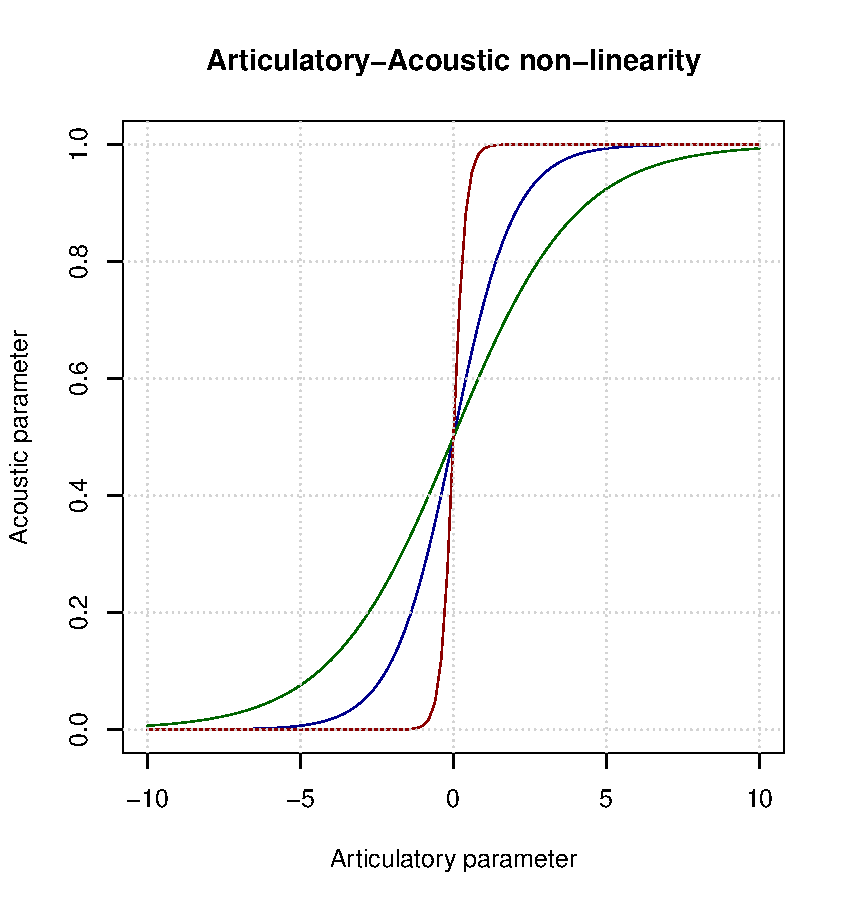
\includegraphics[scale=0.80]{sigmoid.pdf}
\label{Fig.1}
\end{figure}
\subsection{Acoustic-to-Articulatory mapping}
Acoustic-to-Articulatory mapping refers to a special class of the speech inversion problem where simultaneous articulatory and acoustic data is used to learn a mapping between the parameters. This learning, due to the essential non-linear relationship between the parameters, therefore, is also learning of various non-linearities. Recovering articulatory features from acoustics, therefore, remains a non-trivial problem.
\cite{toutios2003}
\cite{badino2016,canevari2013,cernak2016}
\bibliographystyle{unsrtnat}
\bibliography{llc_biblio}

\end{document}
